%!TEX root = ../tesis.tex
\subsection{Fase 2: Decodificaci\'on}
\label{sec:decoding}

En la fase de decodificaci\'on se utiliza un algoritmo decodificador, que depende de un modelo de lenguaje 
y el modelo ac\'ustico, para obtener la secuencia de palabras m\'as probable en base a los vectores 
de caracter{\'\i}sticas que se calcularon en la etapa anterior. 
Esta secci\'on describe los elementos involucrados en esta transformaci\'on, la cual constituye el paso
final del proceso simplificado del reconocimiento del habla que se pretende presentar.

\subsubsection{Modelo de Lenguaje}
Un modelo de lenguaje busca predecir la probabilidad de una secuencia de palabras pertenecientes a un lenguaje.

Formalmente, sea $V$ el conjunto finito de palabras que componen un lenguaje, tambi\'en conocido como 
vocabulario, y $V^\dag$ el conjunto infinito de oraciones que pueden formarse con palabras pertenecientes 
al vocabulario.

Un modelo de lenguaje \cite{CollinsLanguage} consiste en un conjunto finito $V$ y una funci\'on 
de probabilidad $P(x_1,x_2,\ldots,x_n)$ tal que:
\begin{enumerate}

\item $\forall (x_1,x_2,\ldots,x_n) \in V^\dag, P(x_1,x_2,\ldots,x_n) \ge 0$

\item $\displaystyle \sum_{(x_1,x_2,\ldots,x_n) \in V^\dag} P(x_1,x_2,\ldots,x_n) = 1$
\end{enumerate}


En resumen, un modelo de lenguaje define la probabilidad de ocurrencia de una secuencia de palabras
$x_1,x_2,\ldots,x_n$ para un lenguaje dado.

La t\'ecnica basada en n-gramas es la predominante para construir modelos de lenguaje, 
debido a su simplicidad y efectividad \cite{GaoComparative2010}.
Sea $W^L_1$ una cadena de $L $ palabras pertenecientes a un vocabulario $V$ dado. 
Un modelo de lenguaje basado en n-gramas asigna la probabilidad a $W^L_1$ de acuerdo a:

\begin{align}
p(W^L_1) = \displaystyle \prod^L_{i = 1} w_i \mid w^{i - 1}_1 \approx \displaystyle \prod^L_{i = 1} w_i \mid w^{i - 1}_{i - n + 1}
\end{align}

Esta aproximaci\'on se basa en la suposici\'on de Markov de que cada palabra depende solo de las $n - 1$ palabras precedentes, lo cual disminuye significativamente la complejidad del c\'alculo de la probabilidad que se busca para
secuencias de gran longitud.

A modo de ejemplo, se propone la tarea de calcular la probabilidad de la frase \mbox{``El hombre corre''}
utilizando un modelo basado en bigramas ($n=2$).

Sean:
\begin{itemize}
 	\item $\text{\textless} s\text{\textgreater}$ un s{\'\i}mbolo especial utilizado para indicar el inicio 
 	de la secuencia de palabras.
  	\item $\text{\textless} /s\text{\textgreater}$ un s{\'\i}mbolo especial utilizado para indicar el fin 
  	de la secuencia de palabras.
\end{itemize} 

Aplicando la f\'ormula presentada anteriormente, se tiene que:
\begin{equation*}
p(\text{el, hombre, corre}) = p(el \mid \text{\textless} s\text{\textgreater}) \, 
p(\emph{\text{hombre}} \mid el) \, p(corre \mid \emph{\text{hombre}}) \, 
p(\text{\textless} /s\text{\textgreater} \mid corre)
\end{equation*}


Otro tipo de modelo de lenguaje es el basado en una gram\'atica. Las gram\'aticas tienen como ventaja que pueden
utilizarse sin entrenamiento previo. Su principal desventaja est\'a en la dificultad de definir gram\'aticas formales
para lenguajes complejos \cite{Wang2000}.

Un modelo de lenguaje basado en una gram\'atica tradicional asigna una probabilidad de 0 o 1 a cualquier secuencia,
dependiendo de si esta puede o no derivarse a partir de las reglas de la gram\'atica. Sin embargo, si se cuenta con
datos de entrenamiento, es posible asignar una probabilidad a cada regla de modo a mejorar 
la estimaci\'on \cite{huang-handbook10}.

A modo de ejemplo, la siguiente gram\'atica podr{\'\i}a utilizarse como modelo de lenguaje para un sistema simple
de reconocimiento del habla para el acceso a informaci\'on:

\begin{bnf*}
\bnfprod{pregunta}
{\bnfts{Cu\'al} \bnfsp \bnfts{es} \bnfsp \bnfts{la} \bnfpn{info} \bnfsp  \bnfts{en} \bnfsp \bnfpn{ciudad}} \\
\bnfprod{info}
{\bnfts{temperatura} \bnfor \bnfts{presi\'on atmosf\'erica} \bnfor \bnfts{hora}} \\
\bnfprod{ciudad}
{\bnfts{Par{\'\i}s} \bnfor \bnfts{Nueva York} \bnfor \bnfts{Roma}}
\end{bnf*}

\subsubsection{Modelo Ac\'ustico}
El modelo ac\'ustico permite estimar el t\'ermino $P(O|W)$ de la ecuaci\'on \ref{eq:asrFundamental}.
El mismo representa un factor cr{\'\i}tico para la precisi\'on de los resultados obtenidos, y puede decirse que
se trata del componente central de cualquier sistema de reconocimiento del habla \cite{huang-handbook10}.

Es en este elemento del reconocedor en el cual se aplica el concepto de modelos ocultos de Markov que se present\'o
anteriormente. Un modelo ac\'ustico est\'a compuesto por varios modelos ocultos de Markov, cada uno con
los siguientes par\'ametros:


\begin{enumerate}[A)]
	\item \textbf{Estados}


	Un fonema es la unidad b\'asica de sonido capaz de alterar el significado de una palabra \cite{Armbruster2003}.
	Los fonemas a su vez pueden dividirse en unidades subfon\'eticas, las cuales resultan m\'as adecuadas para
	caracterizar las transiciones entre fonemas propias del habla.

	A menudo se elige dividir los fonemas en tres partes para los sistemas de reconocimiento del habla.
	De esta manera, la primera parte depende del fonema anterior, la segunda representa al fonema en cuesti\'on
	y la tercera depende del fonema siguiente \cite{CMUConcepts}.

	Estas unidades fon\'eticas, fonemas o subfonemas, corresponden a los estados del modelo oculto de Markov.
	El decodificador permite obtener la secuencia de estados m\'as probable dada una secuencia de observaciones.
	Esta secuencia de estados $Q$ puede representarse como:

	\begin{align}
		Q = q_1,q_2,q_3,\ldots,o_T\label{eq:hmmQ}
	\end{align}

	Donde:
	\begin{itemize}
		\item $T$ es el n\'umero de observaciones.
		\item $q_1,q_2,q_3,\ldots,q_T \in S$
	\end{itemize}

	La salida del decodificador supone un problema, teniendo en cuenta que el resultado deseado es la secuencia 
	de palabras $W$ de la ecuaci\'on \ref{eq:asrW}, no la de fonemas $Q$.

	El inconveniente anterior se soluciona mediante el diccionario fon\'etico, el cual contiene correspondencias entre palabras y secuencias de fonemas. El mismo forma parte del modelo ac\'ustico \cite{huang-handbook10}.

	\item \textbf{Observaciones}


	Las caracter{\'\i}sticas espectrales de la onda sonora representan los s{\'\i}mbolos observables del habla.
	Los vectores de caracter{\'\i}sticas que se calcularon en la etapa anterior corresponden a las observaciones
	del modelo oculto de Markov.

	Esto es, siendo $O$ la secuencia de observaciones de la ecuaci\'on \ref{eq:asrO} 
	y $V$ el conjunto de s{\'\i}mbolos observables de la ecuaci\'on \ref{eq:hmmV}, $o_1,o_2,o_3,\ldots,o_T \in V$.

	\item \textbf{Distribuciones de Probabilidad}

	Sea $o_t$ el vector de caracter{\'\i}sticas que se observa en el tiempo $t$, es decir, uno de los elementos
	de la ecuaci\'on \ref{eq:asrO}.
	La probabilidad de una observaci\'on como consecuencia de la pronunciaci\'on de un determinado fonema 
	corresponde a la funci\'on $b_j(v_k)$ del modelo oculto de Markov, definida en la ecuaci\'on \ref{eq:hmmB}.
	Por tanto, la probabilidad de observaci\'on de $o_t$ est\'a dada por $b_j(o_t)$ 

	Como un vector de caracter{\'\i}sticas puede tomar un gran n\'umero de valores, los m\'etodos utilizados con
	mayor frecuencia en la actualidad coinciden en tratarlo como una variable continua.

	Una funci\'on de densidad de probabilidad (FDP por sus siglas en ingl\'es) de una variable aleatoria continua describe la probabilidad relativa seg\'un la cual dicha variable aleatoria tomar\'a determinado valor \cite{Evans2011}.

	El m\'etodo m\'as extendido para calcular $b_j(o_t)$ se basa en funciones Gaussianas para definir 
	una FDP \cite{Jurafsky}.
	La versi\'{o}n simple del m\'etodo Gaussiano asume que los valores del vector de observaciones $o_t$ presentan una distribuci\'on normal. Sin entrar en detalles matem\'aticos, se presenta la definici\'on formal 
	de $b_j(o_t)$ para este m\'etodo.

	Sean:

	\begin{itemize}
		\item $\mu_j$ el vector media de la curva Gaussiana.
		\item $\Sigma_j$ la matriz covarianza de la curva Gaussiana.
	\end{itemize}

	\begin{align}
    	b_j(o_t) = \frac{1}{\sqrt{(2\pi)|\Sigma_j|}}e^{[(o_t-\mu_j)'\Sigma_j^{-1}(o_t-\mu_j)]}\label{eq:hmmGaussian}
	\end{align}

	En la pr\'actica, la mayor{\'\i}a de los reconocedores utiliza m\'as de una funci\'on Gaussiana, combinando
	los valores mediante una t\'ecnica conocida como mezclas Gaussianas \cite{huang-handbook10}.

	Existen adem\'as otros m\'etodos para definir la probabilidad de observaci\'on, como la cuantizaci\'on
	vectorial \cite{Burton1983} y las redes neuronales \cite{KristineApplying1995}.

	En general, los par\'ametros probabil{\'\i}sticos del HMM se calculan durante la fase de entrenamiento,
	antes de la utilizaci\'on del sistema de reconocimiento del habla. Estos valores incluyen:

	\begin{itemize}
		\item La probabilidad de observar un determinado fonema al inicio de la oraci\'on: $\pi_i$.
		\item La probabilidad de transici\'on entre fonemas: $a_{ij}$.
		\item Los par\'ametros relacionados a $b_j(v_k)$. 

		En el caso del m\'etodo Gaussiano simple: los par\'ametros $\mu_j$ y $\Sigma_j$ de la 
		ecuaci\'on \ref{eq:hmmGaussian}.
	\end{itemize}

\end{enumerate}

\begin{figure}[H] 
\centering
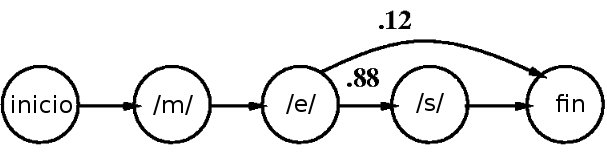
\includegraphics[width=0.5\textwidth]{./graphics/hmm_palabra.png}
\caption{Posible representaci\'on ac\'ustica de la palabra ``mes''. }
\label{figure:hmm-palabra}
\end{figure}

La cantidad de modelos ocultos de Markov depende del enfoque del modelo ac\'ustico, pudiendo darse 
que \cite{Livescu2012}:

\begin{itemize}
 	\item El modelo define un HMM por palabra:


 		Este tipo de modelo requiere de ejemplos de pronunciaci\'on de cada palabra del lenguaje para 
 		su entrenamiento, por lo cual es raramente utilizado en la pr\'actica.
 	\item El modelo define un HMM por fonema:


 		Este tipo de modelo permite el reconocimiento
 		de palabras para las cuales no se cuenta con ejemplos de pronunciaci\'on.
 	\item El modelo define un HMM por fonema, dependiendo del contexto:


 		El sonido particular de un fonema puede variar de acuerdo al fonema anterior y al siguiente.
 		Este tipo de modelo define un HMM para cada una de esas variaciones, y es utilizado
 		en la mayor{\'\i}a de los sistemas de reconocimiento del habla \cite{Odell95theuse}.
 \end{itemize}  

\subsubsection{Espacio de B\'usqueda}
El objetivo de la fase de decodificaci\'on puede ser considerado esencialmente como un problema de 
b\'usqueda \cite{huang-handbook10}.
El algoritmo decodificador intenta encontrar la secuencia de estados m\'as probable dada la secuencia de
vectores de caracter{\'\i}sticas que recibe como entrada, en un \'unico HMM que constituye su espacio de b\'usqueda.

Teniendo en cuenta que el modelo ac\'ustico est\'a constituido por varios modelos ocultos de Markov, se plantea
la necesidad de definir un \'unico HMM para el algoritmo decodificador. Suponiendo que el modelo ac\'ustico define
un HMM por fonema, esto puede hacerse de la siguiente manera:

\begin{enumerate}
	\item Se concatenan los modelos ocultos de Markov de los fonemas de manera a obtener un HMM por cada palabra. 
	La probabilidad de transici\'on entre fonemas est\'a dada por el diccionario fon\'etico.
	\item Se concatenan los modelos ocultos de Markov de las palabras de manera a obtener un \'unico HMM que
	constituye el espacio de b\'usqueda. La probabilidad de transici\'on entre palabras est\'a dada por el modelo
	de lenguaje.
\end{enumerate}

\begin{figure}[H] 
\centering
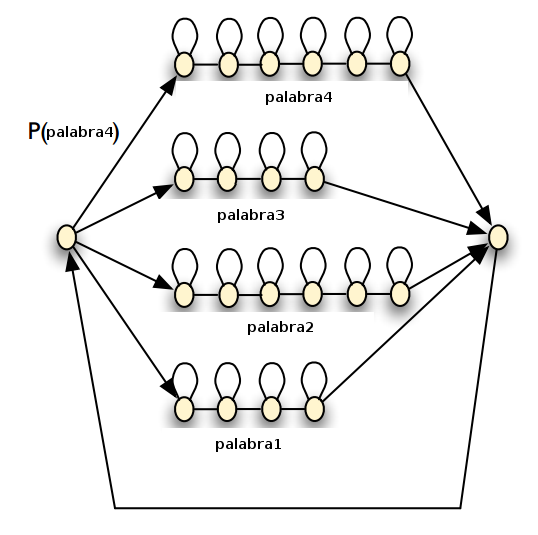
\includegraphics[width=0.5\textwidth]{./graphics/espacio.png}
\caption{Espacio de b\'usqueda para un lenguaje simple de cuatro palabras. }
\label{figure:espacio-busqueda}
\end{figure}



\subsubsection{Algoritmo de Viterbi}
Una vez calculados los vectores de caracter{\'\i}sticas, y habiendo construido el espacio de b\'usqueda, se cuenta con
todos los elementos necesarios para el algoritmo decodificador. Un algoritmo frecuentemente utilizado para
la decodificaci\'on se denomina algoritmo de Viterbi.

El algoritmo de Viterbi, tomando como entrada una secuencia de observaciones y un \'unico aut\'omata, 
encuentra el camino \'optimo a trav\'es del aut\'omata, esto es, la mejor secuencia de estados. 
La descripci\'on y el pseudoc\'odigo que se presentan en esta secci\'on
est\'an basados principalmente en \cite{Jurafsky, Rabiner89atutorial}.

M\'as formalmente, se busca la mejor secuencia de estados $Q = (q_1,q_2,\ldots,q_T)$ 
dadas una secuencia de observaciones $O = (o_1,o_2,\ldots,o_T)$ y un modelo $\lambda$.

El algoritmo utiliza una matriz de probabilidades $viterbi$, donde cada celda $viterbi[i,t]$ 
contiene la probabilidad del mejor camino teniendo en cuenta las $t$ primeras observaciones y 
terminando en el estado $i$ del modelo. Esto es:

\begin{align}
	viterbi[i,t] = \displaystyle \max_{q_1,q_2,\ldots,q_{t - 1}} P(q1,q2,\ldots,q_{t - 1},
		q_t = i,o_1,o_2,\ldots,o_t \mid \lambda) 	
\end{align} 

Para calcular los valores de $viterbi[i,t]$, el algoritmo de Viterbi asume la invariante de la 
programaci\'on din\'amica. Esto es, se asume que si el mejor camino para una secuencia de observaciones 
pasa por un estado $q_i$, entonces este camino incluye el mejor camino hasta $q_i$ inclusive. 
Este supuesto, aunque no siempre sea correcto, permite descomponer el problema y simplificar su soluci\'on,
mediante la siguiente relaci\'on de recurrencia:

\begin{align}
	viterbi[i,t] = \displaystyle \max_i (viterbi[i,t-1]a_{i,j})b_j(o_t)
\end{align}

\begin{algorithm}[H]
\caption{Algoritmo de Viterbi} \label{viterbi}
\begin{algorithmic}[1]
\REQUIRE $observaciones$ de longitud $T$, $grafo\mbox{-}estados$.
\ENSURE $estados$, el mejor camino.
\STATE $num\mbox{-}estados \leftarrow$ CANTIDAD-DE-ESTADOS($grafo\mbox{-}estados$) 
\STATE Crear una matriz de probabilidades $viterbi[num\mbox{-}estados, T]$
\FOR{cada estado $s$ desde $0$ hasta $num\mbox{-}estados$}
	\STATE $viterbi[s,0] = \pi_s$
\ENDFOR
\FOR{cada paso $t$ desde $0$ hasta $T - 1$}
	\FOR{cada estado $s$ desde $0$ hasta $num\mbox{-}estados$}
		\FOR{cada transici\'on $s$ desde s especificada por el $grafo\mbox{-}estados$}
		\STATE $nuevo\mbox{-}puntaje \leftarrow viterbi[s,t] * a[s,s'] * b_{s'}[o_t]$
		\IF{$viterbi[s',t+1] = 0 \parallel nuevo\mbox{-}puntaje > viterbi[s',t+1]$}
			\STATE $viterbi[s',t+1] \leftarrow nuevo\mbox{-}puntaje$
			\STATE $puntero\mbox{-}retroceso[s',t+1] \leftarrow s$
		\ENDIF  
		\ENDFOR
	\ENDFOR
\ENDFOR
\STATE $estados \leftarrow$ retroceso desde la celda con mayor valor en la \'ultima columna de $viterbi[]$
\\ \COMMENT{Usando $puntero-retroceso$}.
\RETURN $estados$
\end{algorithmic}
\end{algorithm}

El algoritmo de Viterbi procesa por completo el tiempo $t$ antes de continuar con el tiempo $t + 1$, por
lo cual se dice que es un algoritmo s{\'\i}ncrono en el tiempo \cite{huang-handbook10}.

En la pr\'actica, para vocabularios extensos, el espacio de b\'usqueda resulta demasiado grande.
Como soluci\'on a este problema suelen podarse los caminos poco probables en cada tiempo $t$,
utilizando una t\'ecnica conocida como b\'usqueda en haz \cite{Jurafsky}.

Otro algoritmo que puede utilizarse para la decodificaci\'on es el algoritmo A*. Este algoritmo
utiliza una funci\'on heur{\'\i}stica, que debe definirse, para elegir los caminos a expandir
durante el proceso de b\'usqueda \cite{Russell2003Solving}. 
El problema de definir una heur{\'\i}stica adecuada a\'un no ha sido resuelto, aunque existen soluciones propuestas.

El algoritmo A* puede calcular probabilidades correspondientes al tiempo $t + 1$ sin haber completado 
las del tiempo $t$, por lo cual es considerado un algoritmo as{\'\i}ncrono en el tiempo.

Con una heur{\'\i}stica adecuada, el algoritmo A* puede utilizarse para espacios de b\'usqueda 
muy grandes \cite{huang-handbook10}.
A\'un as{\'\i}, el algoritmo de Viterbi con b\'usqueda en haz es el m\'etodo utilizado con mayor frecuencia
en los sistemas de reconocimiento del habla \cite{huang-handbook10}. 
Esto se debe principalmente a la ventaja en cuanto a eficiencia relacionada a la b\'usqueda s{\'\i}ncrona 
en el tiempo \cite{huang-handbook10}.

La salida de la fase de decodificaci\'on es la secuencia de palabras m\'as probable dados los vectores
de caracter{\'\i}sticas espectrales, los cuales se calcularon en base a la entrada ac\'ustica durante
la fase de extracci\'on de caracter{\'\i}sticas. Con esto llega a su culminaci\'on el proceso b\'asico
del reconocimiento del habla.